%%%%%%%%%%%%%%%%%%%%%%%%%%%%%%%%%%%%%%%%%%%%%%%%%%%%%%%%%%%%%%%%%%%%%
% LaTeX Template: Project Titlepage Modified (v 0.1) by rcx
%
% Original Source: http://www.howtotex.com
% Date: February 2014
% 
% This is a title page template which be used for articles & reports.
% 
% This is the modified version of the original Latex template from
% aforementioned website.
% 
%%%%%%%%%%%%%%%%%%%%%%%%%%%%%%%%%%%%%%%%%%%%%%%%%%%%%%%%%%%%%%%%%%%%%%

\documentclass[10pt]{report}

% packages to be used
\usepackage[a4paper]{geometry}
\usepackage[myheadings]{fullpage}
\usepackage{fancyhdr}
\usepackage{lastpage}
\usepackage{graphicx, wrapfig, subcaption, setspace, booktabs}
\usepackage[T1]{fontenc}
\usepackage[font=small, labelfont=bf]{caption}
\usepackage{fourier}
\usepackage[protrusion=true, expansion=true]{microtype}
\usepackage[english]{babel}
\usepackage{sectsty}
\usepackage{url, lipsum}
%\usepackage{pythonhighlight}
\usepackage{mathtools}
\usepackage{amsmath} % to feed new lines in equation
\usepackage{hyperref} % added to reference figures with the string Fig
\usepackage{amssymb} % to introduce reverse triangle symbol
% \usepackage{natbib} % to give author name while citation

\usepackage{color}


\usepackage[nottoc,numbib,section]{tocbibind}

% Additional comments
\DeclarePairedDelimiter\ceil{\lceil}{\rceil}
\DeclarePairedDelimiter\floor{\lfloor}{\rfloor}
\newcommand{\HRule}[1]{\rule{\linewidth}{#1}}
\onehalfspacing
\setcounter{tocdepth}{5}
\setcounter{secnumdepth}{5}
\renewcommand{\thesection}{\Roman{section}} % added to make the numbering in % sections to roman numerals

%-------------------------------------------------------------------------------
% HEADER & FOOTER
%-------------------------------------------------------------------------------
\pagestyle{fancy}
\fancyhf{}
\setlength\headheight{15pt}
\fancyhead[L]{Lab Rotation}
\rhead{ \thepage}

%-------------------------------------------------------------------------------
% TITLE PAGE
%-------------------------------------------------------------------------------

\begin{document}

\title{ \normalsize \textsc{Lab Rotation}
		\\ [2.0cm]
		\HRule{0.5pt} \\
		\LARGE \textbf{\uppercase{Image Reconstruction Using\\Neuromorphic Cameras}}
		\HRule{2pt} \\ [0.5cm]
		\normalsize  \vspace*{5\baselineskip}}

\author{
		Sudeshna Bora\\
        Guided By - Prof. Dr. Guillermo Gallego\\
Bernstein Center for Computational Neuroscience, Berlin}

\maketitle

\newpage

\tableofcontents

\newpage
\setcounter{page}{1} % added to start page number from 1
\section{Abstract}
Neuromorphic cameras (also called event-based cameras) are a paradigm shift from conventional cameras and provides potential advantages over conventional frame-based cameras (high speed, high dynamic range, low power consumption) \cite{Gallego20pami}. 
Due to their different way of acquiring and storing visual data, the algorithms used for event-based processing are also markedly different. 
My lab rotation focuses on the task of image intensity reconstruction algorithms from event data. 
This is a quasi theoretical lab rotation which focuses on the following deliverable. 
First, I provide an introduction to event-based cameras (\autoref{sec:introduction})
and review the literature on image reconstruction algorithms in this paradigm (\autoref{sec:literature}). 
Then I decide to focus on comparing two methods.
For the first one, I implement the unsupervised sparse dictionary learning algorithm proposed by Barua et. al. \cite{Barua16wacv} (\autoref{sec:dictionary-learning}), since it is not publicly available. 
As second algorithm, I use the convolutional recurrent neural network proposed by Scheerlinck et. al. \cite{Scheerlinck20wacv} (\autoref{sec:firenet}). 
In conclusion, this report focuses on our findings from the implementation of the first algorithm and on a comparative analysis of the two algorithms (\autoref{sec:discussions}).


\section{Introduction}
\label{sec:introduction}
Neuromorphic (i.e., event-based) cameras are biologically inspired visual sensors that unlike traditional cameras do not capture entire intensity of the visual space at a given time. 
Instead, the pixels of these sensors work independently (there is no global or rolling shutter) and capture any change in brightness (or ``intensity'') that is sensed at the photoreceptor (actually, the logarithm of brightness) if it is greater than a certain threshold \cite{Boahen05sa}. 
These pixel-wise intensity changes are called ``events'' and they are timestamp with very high temporal resolution (in the order of microseconds).
\autoref{fig:difference} illustrates the different working principles of frame-based and event-based cameras.
The asynchronous nature and sensitivity to scene dynamics makes neuromorphic event cameras superior to conventional cameras in terms of low latency, high temporal resolution, high dynamic range and low power consumption.

The first neuromorphic camera was developed by Mahowald and Mead \cite{Mahowald91sciamer}. 
The Dynamic Vision Sensor (DVS) \cite{Lichtsteiner08ssc}, 
the Asynchronous Time-based Image Sensor (ATIS) \cite{Posch11ssc} 
and the Dynamic and Active Pixel Vision Sensor (DAVIS) \cite{Brandli14ssc} are the three main event camera designs. 
The DVS is inspired by the transient visual pathway till the ganglion cells (dorsal stream). 
The ATIS, has in addition to the DVS output, grayscale events that are inspired by the ``what'' visual pathway through the parvo layer of the brain (ventral stream) \cite{Posch14ieee}. 
The DAVIS combines a DVS with a synchronous frame-based camera, on the same pixel array.
The workings of the event camera can be juxtaposed to the flow of stimuli from visual receptive field to deeper brain layers with the help of neurons that fire if the incoming stimuli is above a threshold. 
Similarly, spikes (events) are produced by pixels of the event camera when a threshold is crossed. 
This information then travels from the first layer to deeper layers of the camera circuitry.
% The pathways: https://en.wikipedia.org/wiki/Two-streams_hypothesis

\begin{figure}
\centering
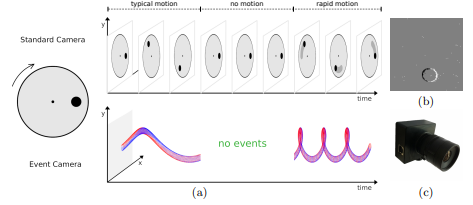
\includegraphics[width=.8\linewidth]{eccv.PNG}
  \caption{Difference between traditional camera (top) and event-based camera (bottom) when they both view a small black circle on a rotating disk.
  The traditional (video) camera acquires frames at a constant rate regardless of what happens in the scene.
  By contrast, in the event-based camera only the pixels that \emph{change intensity} (i.e., those corresponding to the moving edges of the black circle) produce an output; in this case, a ``spiral'' of events in space-time.
  Image courtesy of~\cite{Kim16eccv}.}
  \label{fig:difference}
\end{figure}


\subsection{Working Principle of Event-based Cameras}
\label{sec:working-principle-events}
This subsection develops a mathematical model to describe how an event-based camera works (and the output that it produces). 

As stated above, event-based cameras respond to brightness changes in the scene asynchronously and independently for every pixel. 
Each pixel memorizes the log intensity (log photocurrent $L = \log(I)$) each time it sends an event, and continuously monitors for a change of sufficient magnitude from this memorized value to trigger the next event. 
Ideally in the noiseless case, an event $e_{k}$, which is described by a tuple ($X_{k},t_{k},p_{k}$), 
is triggered at pixel location $X_{k} = (x_{k},y_{k})^{\top}$ at time $t_{k}$ as soon as the brightness increment since the last event at that pixel, 
\begin{equation}
  \Delta L(X_{k},t_{k}) \doteq L(X_{k},t_{k}) - L(X_{k},t_{k} - \Delta t_{k}),
  \label{eq:event-camera}
\end{equation}
crosses a threshold $C>0$:
\begin{equation}
    \Delta L(X_{k},t_{k}) = p_{k} C.
    \label{eq:threshold}
\end{equation}
Here, $\Delta t_{k}$ is the time since the last event, $p_{k} \in \{+1,-1\}$ is the polarity signifying the sign of brightness change \cite{Lichtsteiner08ssc}
(positive if there was a brightness increase --also called ON event--, and negative if there was a brightness decrease --an OFF event--). 
The threshold or contrast sensitivity $C$ is determined by the pixel bias currents \cite{Xu17cvpr,Nozaki17ted} which set the speed and threshold
voltages of the change detector. 
Positive and negative events may be triggered according to different thresholds. 

\textbf{Linearized Event Generation Model}. 
For small $\Delta t_{k}$, \autoref{eq:event-camera} can be approximated using Taylor's expansion $\Delta L(X_{k},t_{k}) \approx \frac{\partial L}{\partial t}(X_{k},t_{k}) \Delta t_{k}$ , thus the events can be interpreted as the temporal derivative: 
\begin{equation}
    \frac{\partial L}{\partial t} (X_{k},t_{k}) \;\approx\; \frac{p_{k}C}{\Delta t_{k}}
\end{equation}

Approximating \autoref{eq:threshold} under brightness constancy assumption and small $\Delta t_{k}$ gives us
\begin{equation}
    \Delta L \approx - \nabla L \cdot v\, \Delta t_k.
\end{equation}
This equation states that the brightness change was produced by a brightness gradient $\nabla L (X_{k},t_{k}) = (\partial_{x} L , \partial_{y} L )^{\top}$ (i.e., an edge) moving with velocity $v$ on the image plane during a time $\Delta t_k$, that is, over a displacement $\Delta x = v \Delta t_k$. 
No events are generated when the motion is parallel to the edge (as implied by the dot product in the formula) and fastest events (minimal time) are generated if the motion is perpendicular to the edge \cite{Bryner19icra}.

\textbf{Noise Model}. 
The above equations are idealized and do not account for sensor noise and transistor mismatch. 
A more realistic model accounts for the stochasticity of the model and can be represented by a probability function of local illumination level and sensor parameters. 
The DVS \cite{Lichtsteiner08ssc} paper suggests a noise model described by a Gaussian distribution centered at the contrast threshold $C$. 
There are other, more complicated, probabilistic models that account for the likelihood of event generation as being proportional to the magnitude of the image gradient \cite{Censi14icra} or being modeled by a mixture distribution in order to be robust to sensor noise \cite{Gallego17pami}.


\subsection{Event Representation}
\label{sec:event-representation}
The asynchronous event stream produced by event-based cameras is often transformed into alternative, more familiar representations that are compatible with non-spiking algorithms and facilitate the extraction of meaningful information to solve the task at hand. 
In this subsection we discuss some of the forms in which event data are represented. 
Specifically we focus on two event types that will be used in \autoref{sec:description}. 

The simplest representation is the individual events $e_{k} = \{ X_{k},t_{k},p_{k}\}$. 
As these do not provide much information on the event/visual field; it is used conjointly with probabilistic filters or SNN which has additional events information stored \cite{Gallego17pami}.
In order to aggregate the spatial and temporal information from multiple events, event packets and frame/2D histogram are used. 
Events $\mathcal{E} = \{e_{k}\}_{k=1}^{N_{e}}$ in a spatio-temporal neighbourhood are processed together in an event packet. 
These packets are then converted to an image to form a 2D histogram. 
Based on spatio-temporal neighbourhood characterisation, other forms of representations have been developed like Time Surfaces\cite{Delbruck08issle}, 3D point sets \cite{Benosman14tnnls} or 2D point sets on the image plane \cite{Ni12tro}.

Event data can be represented by summing the number of events at each pixel (event frame or 2D polarity histogram, also called brightness increment image).
However this representation decreases the performance in case of large motions (i.e., large event accumulation). 
Event frames can be motion-compensated \cite{Gallego17ral} when combined with a motion hypothesis.
To mitigate the above decrease in performance (i.e., to decrease information loss due to accumulation), Zhu et.al \cite{Zhu18rss} and Ye et. al \cite{Ye19arxiv} proposed to combine even frames (which count the number of events per pixel) and time surfaces (which record the timestamp of the last event at each pixel). 
This combined representation was used to train artificial neural networks that learned to estimate these motion (optical flow) in self- and unsupervised manners.

Building on top of it, Zhu. et. al \cite{Zhu19cvpr} proposed event tensors or ``voxel grids''.
Voxel grids or 3D histograms are a better representation than 2D histograms because they preserve better temporal information. 
A voxel grid is a 3D histogram where each voxel represents a particular pixel and timestamp. 
Each event's polarity can be accumulated on a voxel or spread among closest voxels using a kernel $\kappa$ (weighted accumulation). 
Barua et. al's algorithm (\autoref{sec:dictionary-learning}) used $m$ consecutive event frames to represent the event data, which is equivalent to a zero-th order interpolated voxel grid with $m$ time slices. 

If there are $N$ input events and $B$ temporal bins (slices) in the voxel grid, the timestamps of the events are scaled to the rage $[0, B - 1]$ using the simple formula $t_i \mapsto b_i$:
\begin{equation}
b_{i} = (B - 1)\frac{t_{i} - t_{1}}{t_{N} - t_{1}}.
\end{equation}
Now each event has integer coordinates ($x_i, y_i$), and a fractional coordinate $b_{i} \in [0, B - 1]$. 
Events are accumulated in the voxel grid (volume) $V$ according to formula:
\begin{align}
V(x, y, b) & = \sum_{i=1}^{N} p_{i} \, \delta(x - x_{i})\, \delta(y - y_{i}) \, \kappa(b - b_{i}), \label{eq:voxel-voting}\\
\kappa(a) & = \max(0, 1 - |a|) \label{eq:voxel-voting:linear-kernel}
\end{align}
Where $\delta$ is the Kronecker delta. 
If the $x_i,y_i$ coordinates of the events were real numbers, due to, e.g., a camera lens undistortion procedure, then the kernel $\kappa$ would be applied to these spatial coordinates, too. 
Otherwise, it is not necessary since they are already integer values and the Kronecker delta suffices.
In the formula above, $V$ is a discretized volume, of dimensions $W \times H \times B$ (image with, image height, number of time bins).
In the tensors, the time domain is treated as channels of traditional images. 2D convolution are performed across the $x, y$ spatial dimensions. 
As we will mention in \autoref{sec:description}, Scheerlinck et. al. \cite{Scheerlinck20wacv} use voxel grids to represent event data that is fed to their artificial neural network.


\section{Literature Review of Image Reconstruction from Event Cameras}
\label{sec:literature}
Reconstructed brightness images act as an interface between event cameras and conventional computer vision algorithms. 
Rebecq et al. \cite{Rebecq19cvpr} have shown that conventional, frame-based algorithms when applied on reconstructed images perform superior to dedicated event algorithms in classification and visual inertia odometry. Additionally, reconstruction of image aids human with visualization and interpretation. This section deals with the history of development of image reconstruction algorithms with an aim to provide chronological view of the development in this area. 

The initial algorithms \cite{Cook11ijcnn} \cite{Kim14bmvc} for image reconstruction worked under the motion restriction of rotational camera motion, static scene and brightness constancy. These algorithms employed message passing between pixels in a network to jointly estimate characteristics. Kalman filter was used on the pixels to estimate brightness gradient and then poisson reconstruction was used to give absolute brightness. Motion restriction was replaced by using variational frameworks with penalty terms. These regularising assumptions \cite{Manderscheid19cvpr} enabled reconstruction for motions and scenes. Temporal smoothing \cite{Rose73book} for reconstruction and fusion of events and frames did away with spatial regularization and also reduced noise and artefacts. Currently, data driven deep learning algorithms \cite{Rebecq19pami} \cite{Mueggler17bmvc} are used in reconstruction. They have been able to produce more natural looking images and mitigate visual artefacts.

\section{Description of the Model and Results}
\label{sec:description}

\subsection[Image Reconstruction Using Sparse Dictionary Learning]{Image Reconstruction Using Sparse Dictionary Learning\footnote{ url for implementation : https://github.com/SudeshnaBora/Computer\_Vision/tree/master/code }}
\label{sec:dictionary-learning}

The first algorithm \cite{Barua16wacv} is a sparse dictionary learning algorithm. 
It develops a patch-based model for event streams by training an over-complete dictionary.
For the input dataset, we generated events using the event camera simulator, ESIM \cite{Rebecq18corl}.
The following algorithm \cite{Barua16wacv} (additionally with an offset) was also used to create events for each pixel from a reference image.\vspace{1ex}

\fbox{%
  \parbox{\textwidth}{%
  \textbf{Input:} threshold $\tau$, number of frames $m$, pixel intensity for the original image $v_{0}$\\
  $r = v_{0}$\\
  for i = 1 to m do\\
      \-\hspace{0.5cm}if $v_{i} > r$ then\\
      \-\hspace{1cm}$E_{p_{i}} = \lfloor{\log_{\tau}\frac{v_{i} + \text{offset}}{r}}\rfloor$\\
      \-\hspace{1cm}$r = \tau^{E_{p_{i}}} \, r$\\
      \-\hspace{0.5cm}else\\
      \-\hspace{1cm}$E_{n_{i}} = \lceil{\log_{\tau}\frac{v_{i} +\text{offset}}{r}}\rceil$\\
      \-\hspace{1cm}$r = \tau^{E_{n_{i}}} \, r$\\
      \-\hspace{0.5cm}end if\\
 end for\\
 \textbf{Output:} event data $E_{p}$ and $E_{n}$
    }%
    \label{Algorithm : Event-creation}
}
\vspace{1ex}

The events were converted into a voxel grid. The polarity in a voxel grid was determined by linear voting of adjacent voxels. 
\autoref{fig:events} shows the results of the event generation algorithm (\autoref{fig:positive event}) used in ESIM and by the above stated \autoref{Algorithm : Event-creation}, for one of the time slices of the voxel grid. 
Moving forward we would be using the events generated from the simulator ESIM \cite{Rebecq18corl}.

\begin{figure}
\centering
\begin{subfigure}{.45\linewidth}
  \centering
  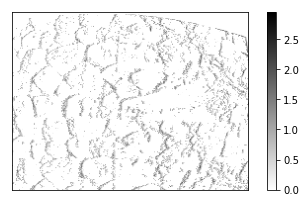
\includegraphics[width=.8\linewidth]{positive_ESIM.PNG}
  \caption{Image of the positive event voxel grid where events are created by ESIM}
  \label{fig:positive event}
\end{subfigure}\;\;
\begin{subfigure}{.45\linewidth}
  \centering
  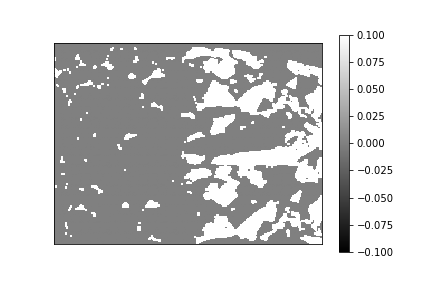
\includegraphics[width=.8\linewidth]{self_event.png}
  \caption{Image of the negative event voxel grid where events are created by Algorithm}
  \label{fig:negative_event}
\end{subfigure}
\caption{Sample time slices of voxel grids of events. 
The texture corresponds to some poster of rocks on a flat wall, as in the \cite{Mueggler17ijrr} dataset. 
The edges that we see represent the borders of those rocks.}
\label{fig:events}
\end{figure}

In the training phase, we computed the $x$ and $y$ gradients of the logarithm of the intensity image. 
The gradients were computed by using two 1-D filters (i.e., applying spatial convolution):
\begin{equation}
    f_{1} = [-1, 1],\quad f_{2} = f_{1}^{T}
\end{equation}

The input dataset contains 100000 patches ($X$) from the gradient and the event frames. 
The first $2n$ rows contain the gradients and the remaining $2mn$ rows contain the events from $m$ frames, where $n$ is the number of pixels in each patch. 
We used the K-SVD algorithm \cite{Aharon06tsp} to train the sparse patch-based dictionary.
That is, we solved the problem:
\begin{equation*}
  \begin{aligned}
    &D^{\ast} = \arg \min_{D,\alpha} || X - D \alpha ||_{2}^{2} \quad\text{s.t.}\quad ||\alpha ||_{0} \leq K_{s},\\
    &D = \begin{bmatrix} D_{g} \\ D_{e} \end{bmatrix}\\
 \end{aligned}
\end{equation*}
where $\alpha$ is vector of sparse coefficient. $K_{s} = 8$. 
\autoref{fig:training} shows the flow of execution for training an over-complete representation of the data.

\begin{figure}
\centering
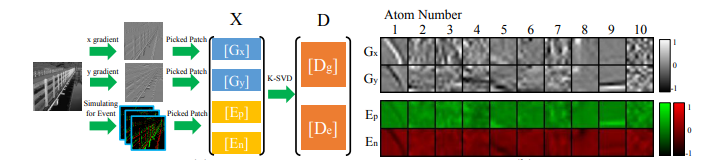
\includegraphics[width=.9\linewidth]{Training.PNG}
  \caption{Training phase using a Dataset. 
  A dictionary of patches $D$ is learned from synthetic data.
  The dictionary consists of atoms. 
  Each atom has a spatial component (the part of the patch corresponding to the $x$ and $y$ image gradients, $G_x, G_y$) 
  and a temporal component (the part of the patch corresponding to the event frames $E_p, E_n$).
  The dictionary is learned by applying the K-SVD clustering algorithm on a large collection of input patches $X$.}
  \label{fig:training}
\end{figure}
    
The learned dictionary $D$ is then used to reconstruct new raw data from the DVS camera. 
The Orthogonal Matching Pursuit (OMP) algorithm \cite{Pati93asilomar} was used on the event data vector to get the sparse coefficient $\alpha$ for a new input event data $Y_e$:
\begin{equation}
    \alpha^{\ast} = \arg \min_{\alpha} \| Y_{e} - D_{e} \alpha \|_{2}^{2} \quad \textrm{s.t.} \quad \|\alpha\|_{0} \leq K_{0}.
\end{equation}
This coefficient vector is a ``sparse code'' representing the input event data in terms of the atoms of the learned event dictionary.
Next, the sparse coefficient is multiplied with the gradient portion of the dictionary to get logarithmic intensity gradient data. 
Poisson reconstruction \cite{Agrawal05iccv} \cite{Agrawal06eccv} is then used to get the recovered logarithmic intensity image from the gradient data, and this image when raised to the power of threshold is used to get the absolute intensity image in linear scale. 
\autoref{fig:testing} shows the reconstruction procedure from raw event data via the learned dictionary.

\begin{figure}
\centering
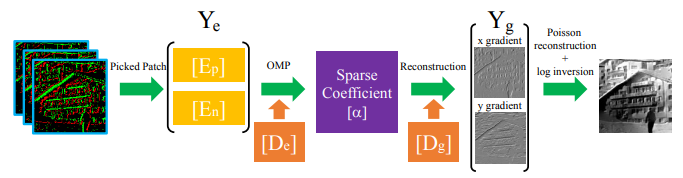
\includegraphics[width=.9\linewidth]{Testing.PNG}
  \caption{Testing phase (i.e., inference): reconstruct an intensity image from raw event data.
  Positive and negative events are converted into a grid-like representation (event frames) $Y_e$.
  Then, using the part of the dictionary corresponding to the events ($D_e$), the sparse coefficient $\alpha$ is computed using the OMP (Orthogonal Matching Pursuit) algorithm. 
  Multiplying this coefficient $\alpha$ by the part of the dictionary corresponding to the spatial gradients ($D_g$) yields gradient patches $Y_g$, with are collected into two images (the $x$ and $y$ gradients). 
  Finally the image gradients are integrated using a Poisson solver to produce the reconstructed absolute intensity.
  }
  \label{fig:testing}
\end{figure}

As can be seen from \autoref{fig:reconstruction} , we were not able to do a perfect reconstruction of the testing dataset. We accord this noisy reconstruction to our learnt dictionary. We believe using a more robust, varied natural images dictionary would have fetched a better result. However, due to time constraint we decided to move forward to the next algorithm. 
\begin{figure}
\centering
\begin{subfigure}{.45\linewidth}
  \centering
  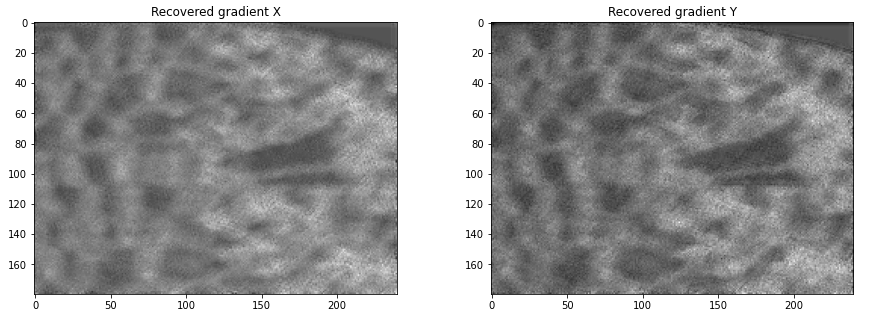
\includegraphics[width=.8\linewidth]{Total_Gradient.PNG}
  \caption{Reconstructed gradient images}
  \label{fig:gradient images}
\end{subfigure}\;\;
\begin{subfigure}{.45\linewidth}
  \centering
  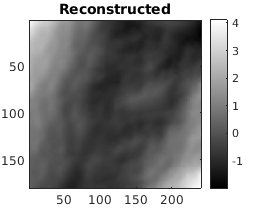
\includegraphics[width=.8\linewidth]{reconstructed.png}
  \caption{Final Reconstructed Image}
  \label{fig:reconstructed}
\end{subfigure}
\caption{Sample of the reconstructed x and y gradients and the final reconstructed image.}
\label{fig:reconstruction}
https://www.overleaf.com/project/5f97f3e5b902930001a447f3\end{figure}

\subsection[Fast Image Reconstruction with Convolutional Neural Network]{Fast Image Reconstruction with Convolutional Neural Network \footnote{ Personal implementation is not maintained in github as it was used for understanding purpose. Url for authors's implementation : https://github.com/cedric-scheerlinck/rpg\_e2vid/tree/cedric/firenet }}
\label{sec:firenet}
The previous algorithm \cite{Barua16wacv} is considered to be the first learning-based method for image reconstruction from event data. 
The current algorithm by Scheerlinck et. al \cite{Scheerlinck20wacv} is a much smaller convolutional network (smaller computational cost) that achieves comparable results with respect to the current state of the art architecture E2VID \cite{Rebecq19pami}.
The algorithm, which is referred to as FireNet, is a fully convolutional recurrent neural network. 
\autoref{fig:firenet} shows the architecture of the network. 
All the layers are $3\times 3$ convolutions except the prediction layer which is $1 \times 1$ convolutions and use ReLU (REctified Linear Unit) activation function. 
The input is a $H \times W \times B$ event tensor with $B = 5$ temporal bins, and sensor height and width as $H$ and $W$ respectively. 
They use linear voting in time to populate the tensor / voxel grid (\autoref{eq:voxel-voting} and \autoref{eq:voxel-voting:linear-kernel}). 
The 5-channel event tensor is fed into the Head layer that has 16 channels. 
This layer is followed by 16 channel convolution gated recurrent (G1, G2) units and 16 channels residual blocks (R1, R2) with skip connections.  
The output is one image per input event tensor.

The loss function used to train this artificial neural network was a weighted sum of reconstruction and temporal loss over  $L$ ( $L = 20$ ) consecutive images.
\begin{equation}
    \mathcal{L} = \sum_{k=0}^{L}\mathcal{L} + \lambda_{TC} \sum_{k = L_{0}}^{L}\mathcal{L}_{k}^{TC}
\end{equation}

The reconstruction loss is calculated by using Perceptual similarity \cite{Zhang18cvprLPIPS} to ground truth image. 
The temporal loss is the photometric error \cite{Rebecq19pami} between two consecutive images. 
The algorithm utilised default ADAM \cite{Kingma15iclr} with learning rate $10^{-4}$ for $1000$ epochs and $\lambda_{TC}$ and $L_{0} = 10$.\autoref{fig:reconstructed-firenet} shows the reconstructed image from event data. AS can be seen, this output shows lesser noise and a more accurate reconstruction.

\begin{figure}
\centering
\begin{subfigure}{.45\linewidth}
  \centering
  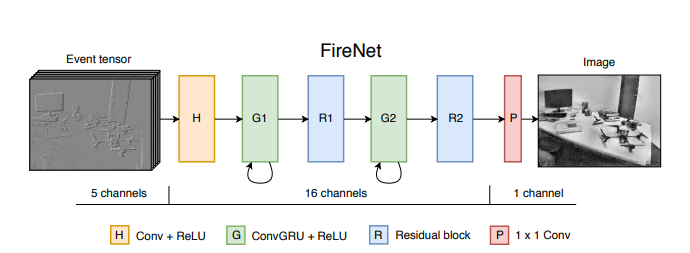
\includegraphics[width=.8\linewidth]{Firenet.PNG}
  \caption{rchitecture of the FireNet artificial neural network. Image courtesy of \cite{Scheerlinck20wacv}.}
  \label{fig:firenet}
\end{subfigure}\;\;
\begin{subfigure}{.45\linewidth}
  \centering
  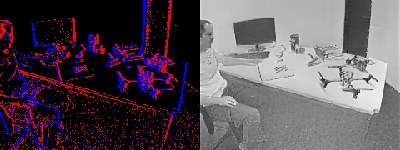
\includegraphics[width=.8\linewidth]{Reconstruction_Firenet.png}
  \caption{Final Reconstructed Image}
  \label{fig:reconstructed-firenet}
\end{subfigure}
\caption{Firenet architecture and output}
\label{fig:reconstruction-firenet}
\end{figure}



\section{Discussions and Conclusions}
\label{sec:discussions}

\textbf{Discussion}.
The two publications \cite{Barua16wacv,Scheerlinck20wacv} do not show results on the same datasets.
Therefore, it is not straightforward to compare their performance.
Notably, FireNet \cite{Scheerlinck20wacv} is based on the latest results on deep learning, and therefore it is expected to perform better than the 4-year earlier work \cite{Barua16wacv}.

From a methodology point of view, Barua et al. \cite{Barua16wacv} perform image reconstruction in two steps: 
First a gradient image is obtained from the events using the learned dictionary and then the gradient is upgraded to absolute intensity using Poisson integration.
The first step is the learning phase, whereas the second step is deterministic.
By contrast, FireNet \cite{Scheerlinck20wacv} performs image reconstruction in one ``single step'', i.e., one artificial neural network; there is no intermediate obvious interpretation of the hidden layers of the neural network; only the output matters.

From a training point of view, both are trained using simulated data. 
FireNet uses supervised learning (the loss function measures the error between the predicted image and the ground truth one).
On the other hand, the method of Barua et al. is based on learning a dictionary using K-SVD, which is a clustering technique (i.e., unsupervised).
FireNet was trained on a larger and probably more diverse dataset, as in \cite{Rebecq19pami}, so it has better data to generalize to unseen scenes.

From an architecture point of view, FireNet has recurrent connections, that is, some sort of memory of past events and reconstructions that can use to produce a better output that if it had no memory. 
By contrast, Barua's method has no memory: once the dictionary has been learned, every $m$ event frames are processed independently, without leveraging past events.
 
Barua's method \cite{Barua16wacv} has 10000 atoms and each atom has 300 dimensions. Thus it has a total of 300k parameters. Whereas, Firenet \cite{Scheerlinck20wacv} has 38k parameters. 

A comparison in terms of speed depends on the particular implementations of the methods.
As far as we know, Barua et al. \cite{Barua16wacv} do not report the runtime of their method.
We used python for prototyping Barua's method and it took several seconds to infer the gradient maps from the input events and the learned dictionary.
By contrast, FireNet is deployed on efficient code that runs on the GPU, so in this regard, the current implementation of FireNet is faster than our re-implementation of Barua's method.

In \textbf{conclusion}, the lab rotation helped me gain knowledge in a completely different field of study as well as in ROS and event simulators. Implementing and comparatively analysing the two algorithms have helped me gain knowledge into niche image processing domains of image reconstruction algorithms, sparse dictionary learning, poisson reconstruction etc.

Looking forward, there are other areas that can be looked onto. One such area is the use of kernelised matrix factorization \cite{fan20arxiv} for learning the dictionary at Barua et. al \cite{Barua16wacv}.
Additionally, we can use layer relevance propagation \cite{Montavon19sip} to visualise which pixels of the input dataset have higher relevance in reconstruction.

% \nocite{*}
\clearpage% or cleardoublepage
%\addcontentsline{toc}{section}{References}
\bibliographystyle{acm}
\bibliography{all}

\end{document}
